\documentclass{sig}

\usepackage{algorithm}
\usepackage{algpseudocode}
\usepackage{amsmath}
\usepackage{appendix}
\usepackage{balance}
\usepackage{caption}
\usepackage{color}
\usepackage{comment}
\usepackage{epstopdf}
\usepackage{graphicx}
\usepackage{listings}
\usepackage{mathtools}
\usepackage{microtype}
\usepackage{multirow}
\usepackage{pdfpages}
\usepackage{subcaption}
\usepackage{subfig}
\usepackage{tabularx}
\usepackage{times}
\usepackage{url}
\usepackage{xcolor}
\usepackage{xspace}
\usepackage{bm}
\usepackage{mdwlist}

\newcommand{\subparagraph}{}
\usepackage{titlesec}

%\titlespacing{\section}{0ex}{0.8ex}{0ex}
%\titlespacing{\subsection}{0ex}{0.8ex}{0ex}
%\titlespacing{\subsubsection}{0ex}{0.7ex}{0ex}
%\setlength{\parskip}{0ex}

\algrenewcommand\alglinenumber[1]{\scriptsize #1:}

\makeatletter
\renewcommand*{\ALG@name}{Investing Rule}
\makeatother


\usepackage{breqn}
\interfootnotelinepenalty=10000

\newcommand{\todo}[1]{\textcolor{blue}{TODO: #1}}
\newcommand{\done}[1]{\textcolor{green}{DONE#1}}
\newcommand{\tim}[1]{\textcolor{red}{Tim: #1}}
\newcommand{\lore}[1]{\textcolor{blue}{Lorenzo: #1}}
\newcommand{\ez}[1]{\textcolor{orange}{ez: #1}}
\newcommand{\sam}[1]{\textcolor{purple}{sam: #1}}
\newcommand{\carsten}[1]{\textcolor{brown}{Carsten: #1}}

\newcommand{\naive}{na\"{\i}ve\xspace}
\newcommand{\Naive}{Na\"{\i}ve\xspace}
\newcommand{\naively}{na\"{\i}vely\xspace}

\newcommand{\ainv}{$\alpha$-investing }
\newcommand{\sfdr}{Sequential-FDR }
\newcommand{\mfdre}{$mFDR_{\eta}$ }
\newcommand{\mfdr}[1]{$mFDR_{#1}$}
\newcommand{\Ex}[1]{E\left[#1\right]}
\newcommand{\Prob}[1]{\text{P}\left(#1\right)}
\newcommand{\CProb}[2]{\text{P}\left(#1|#2\right)}
\newcommand{\pval}{$p$-value }
\newcommand{\pvals}{$p$-values }


\newcommand{\system}{{\sc Aware}}
\newcommand{\Chi}{\mathcal{X}}

\newtheorem{theorem}{Theorem}
\newtheorem{lemma}{Lemma}


%\setlength\abovedisplayskip{0pt plus 2pt minus 0pt}
%\setlength\belowdisplayskip{0pt plus 2pt minus 0pt}

%\makeatletter
%\g@addto@macro \normalsize {%
%\setlength\abovedisplayskip{0pt plus 2pt minus 0pt}%
%\setlength\belowdisplayskip{0pt plus 2pt minus 0pt}%
%\setlength\abovedisplayshortskip{0pt plus 2pt minus 0pt}%
%\setlength\belowdisplayshortskip{0pt plus 2pt minus 0pt}%
%}
%\makeatother

%\makeatletter
%\g@addto@macro \small {%
%\setlength\abovedisplayskip{0pt plus 2pt minus 0pt}%
%\setlength\belowdisplayskip{2pt plus 2pt minus 0pt}%
%\setlength\abovedisplayshortskip{0pt plus 2pt minus 0pt}%
%\setlength\belowdisplayshortskip{2pt plus 2pt minus 0pt}%
%}
%\makeatother

\DeclareMathOperator*{\argmin}{\arg \min}
\DeclarePairedDelimiter\ceil{\lceil}{\rceil}

\captionsetup{font={bf}}

%\newcommand{\system}{{\sc Vizdom}}

\newcommand{\specialcell}[2][c]{
  \begin{tabular}[#1]{@{}c@{}}#2\end{tabular}}

\definecolor{dark-gray}{gray}{0.2}

\newenvironment{packed_item}{
\begin{list}{$\bullet$}{
  \setlength{\itemsep}{-2pt}
  \setlength{\parskip}{1pt}
  \setlength{\labelwidth}{15 pt}
  \setlength{\leftmargin}{10pt}
  \setlength{\itemindent}{0pt}}
}{\end{list}}

% for floated 2 column equations
\newcounter{tempEquationCounter}
\newcounter{thisEquationNumber}
\newenvironment{floatEq}
{\setcounter{thisEquationNumber}{\value{equation}}\addtocounter{equation}{1}% record equation as happened and remember number
\begin{figure*}[t]% float following equation across columns
\normalsize\setcounter{tempEquationCounter}{\value{equation}}% record current equation number in floated location
\setcounter{equation}{\value{thisEquationNumber}}% use previous equation number
}
{\setcounter{equation}{\value{tempEquationCounter}}% set back to equation number in floated location
\hrulefill\vspace*{4pt}% add a horizontal rule separator
\end{figure*}% end float environment
}
\newtheorem{defi}{Definition}
\makeatletter
\newenvironment{subheuristic}[1]{%
  \def\subtheoremcounter{#1}%
  \refstepcounter{#1}%
  \protected@edef\theparentnumber{\csname the#1\endcsname}%
  \setcounter{parentnumber}{\value{#1}}%
  \setcounter{#1}{0}%
  \expandafter\def\csname the#1\endcsname{\theparentnumber\alph{#1}}%
  \ignorespaces
}{%
  \setcounter{\subtheoremcounter}{\value{parentnumber}}%
  \ignorespacesafterend
}
\makeatother
\newcounter{parentnumber}

\newtheorem{heuristic}{Heuristic}

\begin{document}

\title{Aware: Safe Visual Data Exploration}

\numberofauthors{1}
\author{
\alignauthor
%\vspace*{-30pt}
%Paper \#178
\begin{tabular}{cccc}
\end{tabular}\\
%\vspace{1.5mm}
\affaddr{Department of Computer Science, Brown University}\\
%\vspace{0.75mm}
\{firstname\_lastname\}@brown.edu
%\email{\{firstname\_lastname\}@brown.edu}
}

%\numberofauthors{6}
%\author{
%\small{Andrew Crotty, Alex Galakatos, Kayhan Dursun, Tim Kraska, Ugur Cetintemel, Stan Zdonik} \\
%\small{Department of Computer Science, Brown University} \\
%\small{\{crottyan, agg, kayhan, kraskat, ugur, sbz\}@cs.brown.edu}
%}
\date{}
\maketitle

\begin{abstract}
Exploring data via visualizations has become a popular way to understand complex data. Observations derived from the visual results are inherently hypotheses, and thus visually significant information may not carry any statistical significance. Moreover, visual data exploration and recommendation produce observations dynamically, and so result in increasing numbers of false discoveries.  The risk of false discoveries, if not controlled theoretically and systematically, renders visual data exploration unsustainable. To address this problem, we present our solution based on Vizdom~\cite{vizdom}, namely, \system{}, a visual data exploration system that interacts with user to formulate visualization-based hypotheses and provides interactive control of false discoveries based on the recent advance in the subject~\cite{zhao2016controlling}.
\end{abstract}


\section{Introduction}
\label{sec:intro}
In the era of Big Data, interactive data exploration tools arise as an important mean to explore and derive insights from data through visualization.  
However, perceived interesting patterns in visual data representations, such as relationships or trends, may emerge from irrelevant random effects inherent to the data, such as random noises, large variances, insufficient samples, and biases. 
Without proper statistical control, users may mistake a distinct or dominant visual observation as statistically significant.  
On the other hand, systems that search and recommend visualizations automatically based on such interesting visual features further increase the chance of bogus insights.  
A recent study highlights these issues and shows that visualization and recommendation systems that do not consider the risk of false discovery, such as Vizdom~\cite{vizdom}, SeeDB~\cite{seedb} and Data Polygamy~\cite{polygamy}, become difficult to derive insights safely on real-world datasets \cite{binnig2017sustainable}.

False discovery due to random noise is pervasive in visual data exploration on real-world datasets. For example, when using Vizdom~\cite{vizdom} to explore a recently conducted survey on personal habits and opinions~\cite{binnig2017sustainable}, we observed that the preference on watching films on DVD produced visually different proportions of belief in aliens, as shown in Figure~\ref{fig:example} (A and B).
Just by visually examining these charts, users often falsely assumed that people who prefer to watch movies on DVD are more prone to believe in aliens even though this effect is not statistically significant.
%But such predictor proved neither much sensible nor statistically significant.  

Such observation-based hypotheses may be accumulated quickly as the user continues to explore a dataset, and hence dramatically raises the risk of spurious findings. 
With the same survey dataset, after searching through a few different comparisons we stumbled upon a visualization that suggests hair color predicts whether one knows about Michael Stonebraker, and it would be statistically significant if considered as a lone hypothesis. This phenomenon is often referred to as data dredging or $p$-hacking~\cite{head2015extent}, and formally known as the multiple comparison problem~\cite{shaffer1995multiple}.

Several challenges exist to control false insights in such interactive data exploration.  
The first question is what could even be considered as a hypothesis in visual data exploration.
In some cases users might explicitly specify certain hypotheses, but in other instances they do not formulate any hypothesis but still use visualization to infer about the data or to extract an insight.
An ideal system should assist users in hypothesis formulation and corresponding hypothesis test selection.

Second, interactive data exploration mandates that hypotheses are formulated dynamically based on the process of human decision making.  
However the classical statistical procedures such as Bonferroni~\cite{bonferroni1936teoria} and Sequential FDR~\cite{g2016sequential} are not dynamic as they require collecting all the hypotheses a priori before finalizing any significance result.  
Moreover these traditional techniques assume complete pass of the dataset, and thus would make the system non-interactive on larger data.  
Thus an ideal system for interactive control of false discovery should follow progressive computation, which proves to be a more appealing paradigm~\cite{vizdom, onlineagg, zgraggen2016progressive}.  

Finally, parts of the data exploration process can be automated through algorithmic search and recommendation. Such automatic data exploration should also be subject to false discovery control.  

In this demo, we present \system{}\footnote{\system{} stands for Quantifying the Uncertainty in Data Exploration.}, a first ``safe'' visual data exploration tool that addresses these challenges. 
In \system{}, we implemented recent techniques in interactive false discovery control that are both dynamic and progressive~\cite{zhao2016controlling}, apply them to visual data exploration and visualization recommendation, and expose them through a pen- \& touch-based user interface that simplifies and in some cases even automates the creation of hypothesis tests.


%Thus, to address theses challenges, we implemented the recent advance in interactive false discovery control that is both dynamic and progressive, and applied to both visual data exploration and recommendation~\cite{zhao2016controlling}. 

\begin{figure}
\centering
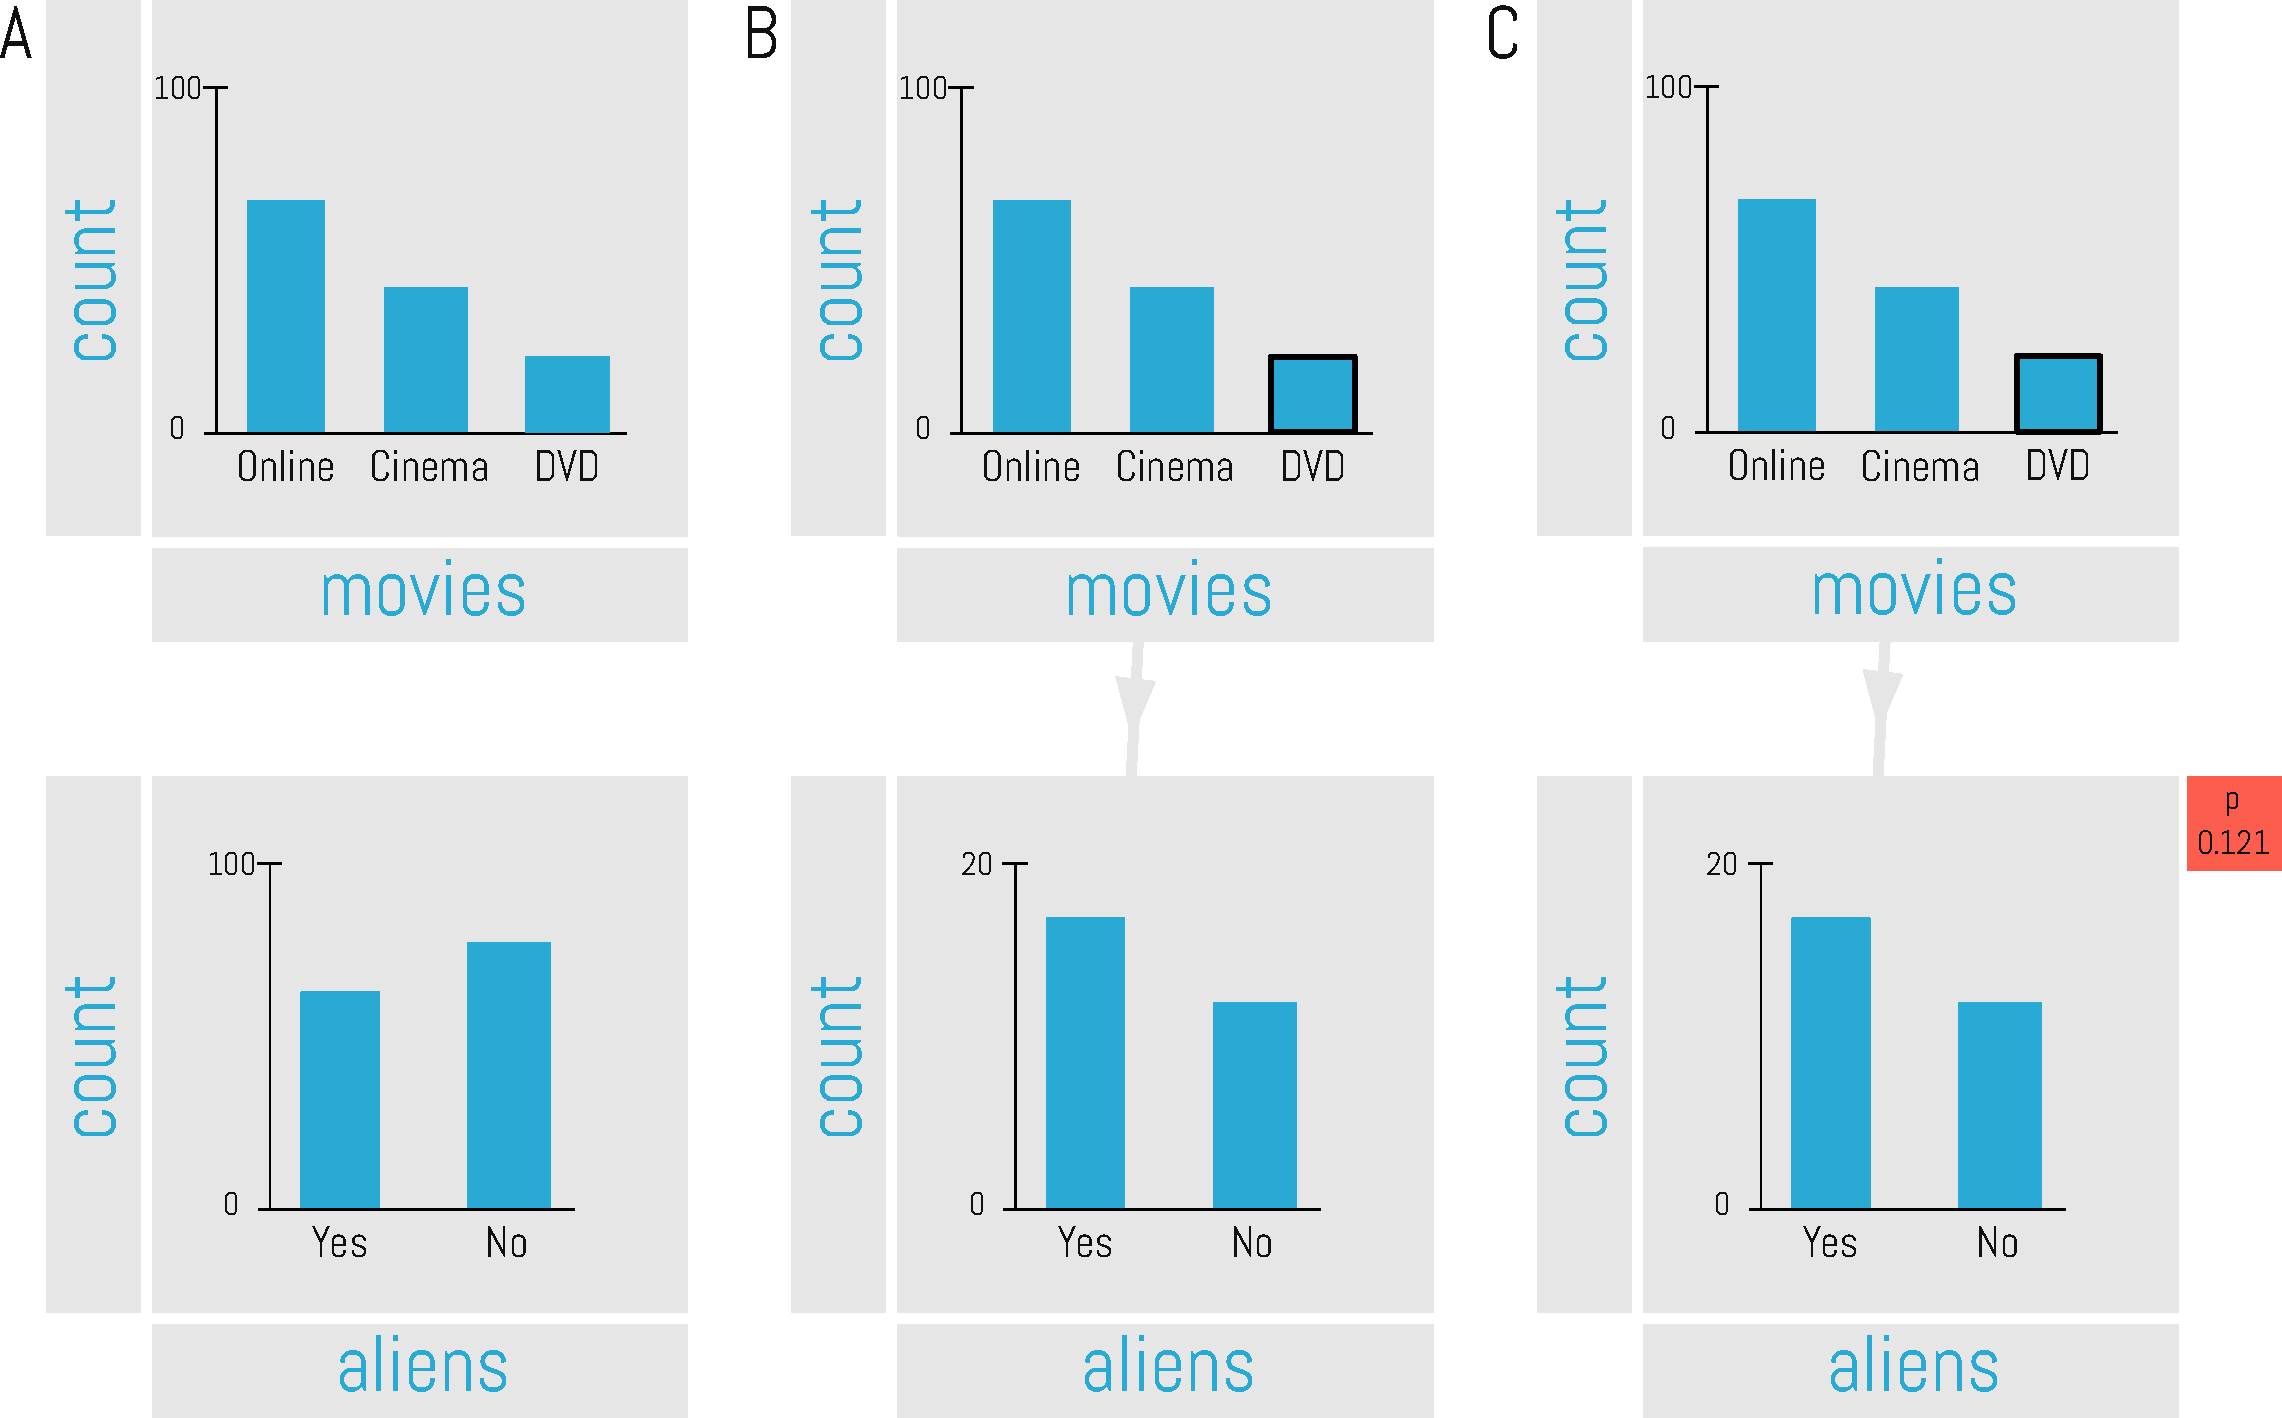
\includegraphics[width=0.47\textwidth]{figures/example}
\caption{Example of a visualization network where users might be led to false discoveries without automatic hypothesis formulation. (A) two separate visualizations showing preferences for watching movies and how many people believe in alien existence; (B) the two visualizations combined where the bottom one shows proportions of belief in alien existence for only people who like to watch movies on DVD, displaying a noticeable difference compared to the overall population. (C) same visualizations as before but now with automatic hypothesis formulation turned on, highlighting that the observed effect is not statistically significant.}
\label{fig:example}
\vspace{-3.5ex}
\end{figure}

\section{Design}
\label{sec:design}
Our design, \system{}, is based on Vizdom~\cite{vizdom} and addresses the aforementioned challenges, namely,
\begin{itemize}
    \item To formulate hypotheses via user interaction;
    \item To visualize the statistical significance and other contextual information for each observation;
    \item To control multiple hypotheses dynamically during data exploration;
    \item To progressively compute the risk of false discovery on larger data.
\end{itemize}

\subsection{Theory}
\label{sec:theory}
The theory of controlling false discovery in interactive data exploration is introduced in~\cite{zhao2016controlling}. Data exploration is treated as a growing sequence of observations.  Each observation is evaluated by a hypothesis test, which outputs a \pval. A false discovery procedure such as $\gamma$-Fixed~\cite{zhao2016controlling} starts with a predefined amount of exploration \textit{budget}, and \textit{invests} a fraction of the budget to each test sequentially.  If the observation is deemed significant, or equivalently, the test is rejected, then a fraction of the investment is returned to the budget. The procedure halts when either the sequence of tests stops or the budget reduces to zero.  The guarantee is that the \textit{marginalized false discovery rate} (mFDR), namely, the ratio of expected number of false discoveries over expected number of all discoveries, is less than the fraction set as the initial exploration budget.

If the exploration budget reaches zero, the per-observation investment can be reduced a posteriori for the past observations.  Because the investment corresponds to the per-test significance level, some previously significant observation may become insignificant, but because the lost of budget is also reduced.  If the reduction of investment regains eventual exploration budget, then the exploration can continue.  Such reduction policy is analogous to the Bonferroni procedure~\cite{bonferroni1936teoria}, where the significance level for each test reduces as more observations are made.

The previously known control procedures such as Bonferroni~\cite{bonferroni1936teoria}, FDR~\cite{BenjaminiH95} and Sequential FDR~\cite{g2016sequential} are not interactive, because the decisions are only finalized when all observations are made.  The main advantage of the \ainv procedures proposed in~\cite{zhao2016controlling} is interactivity in that observations can be made dynamically.

\subsection{User Interface}
\label{sec:ui}

\begin{figure}
\centering
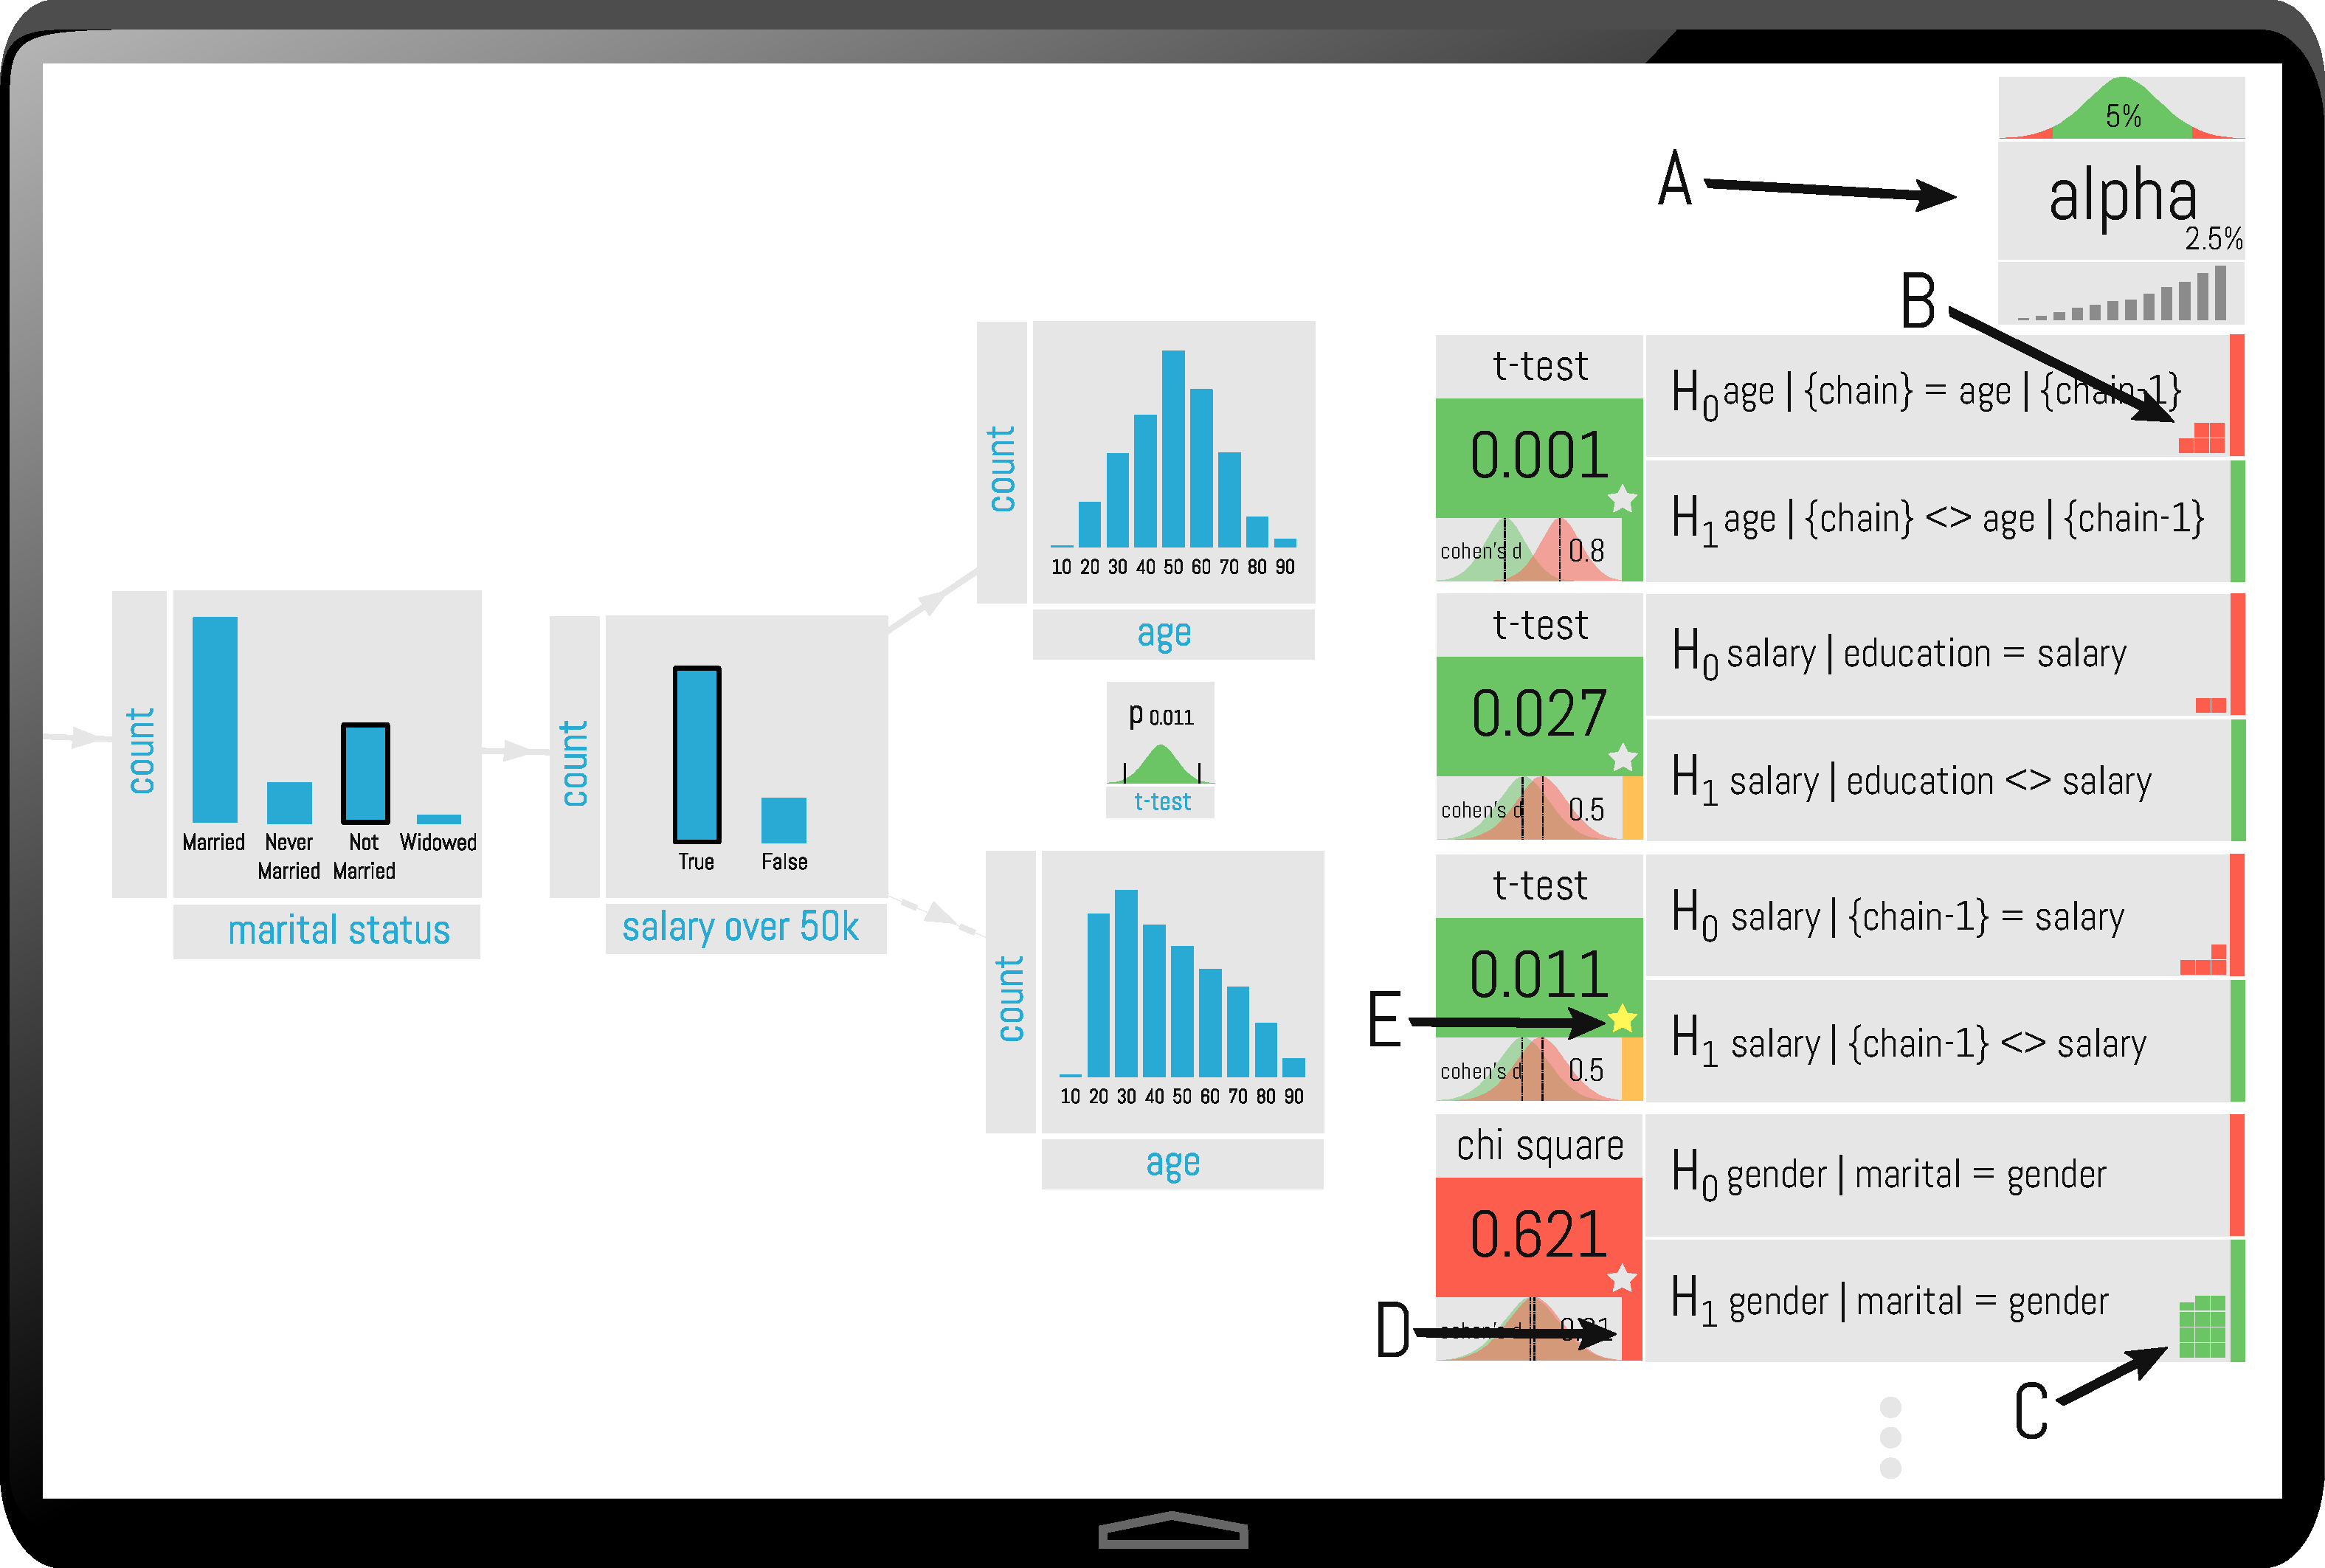
\includegraphics[width=0.48\textwidth]{figures/ui.pdf}
\caption{User Interface}
\label{fig:ui}	
\end{figure}

\system{}'s user interface (UI) features an unbounded 2D canvas where visualizations can be laid out in a free form fashion (Figure~\ref{fig:ui}). It is based on our visual data exploration tool Vizdom~\cite{vizdom} but extended by three new components:

\textbf{Implicit and explicit hypothesis tests:} The 

\textbf{Visualization recommendations:} To speed up the potentially laborious process of manually exploring a dataset we added a visualization recommendation engine. Similar to SeeDB \cite{seedb} our engine allows users to search for filter conditions that have a significant effect (positive or negative) on a given reference visualization. We expose this functionality though a gestural touch UI that can be accessed from any visualization. 

\textbf{Hypotheses tracking:} A ``risk-gauge'' on the right-hand side of the display (A) serves two purposes, namely, to give user a summary of the multiple hypothesis correction procedure (e.g., in this case alpha investing is used with a false discovery rate of 5\% and with current remaining budget of 70\% \sam{revisit this example}), and to provide access to a scrollable list of all the hypotheses that have been explored.
Each list entry can be expanded (in the example all are expanded) to display details about an observation and its statistical significance.  
The text labels describe the null and alternative hypotheses concerning each observation and the corresponding hypothesis test and \pval{}. Each color coded tile indicates whether the observation is statistically significant or insignificant, which corresponds to green or red respectively.  
The distributions of null and alternative hypotheses and the color coded effect size are also visualized (D).  
To help the user understand the effect of data collection, the sample size estimate for the current significance level is displayed for each hypothesis test assuming the effect size is fixed (C).  
For example, the five green squares in (C) indicates approximately five times the current data size with the same effect size would make this observation significant.
Finally, important observations can be marked by tapping the ``star'' icons (E).

\subsection{Backend}
\label{sec:backend}

\begin{figure}
\centering
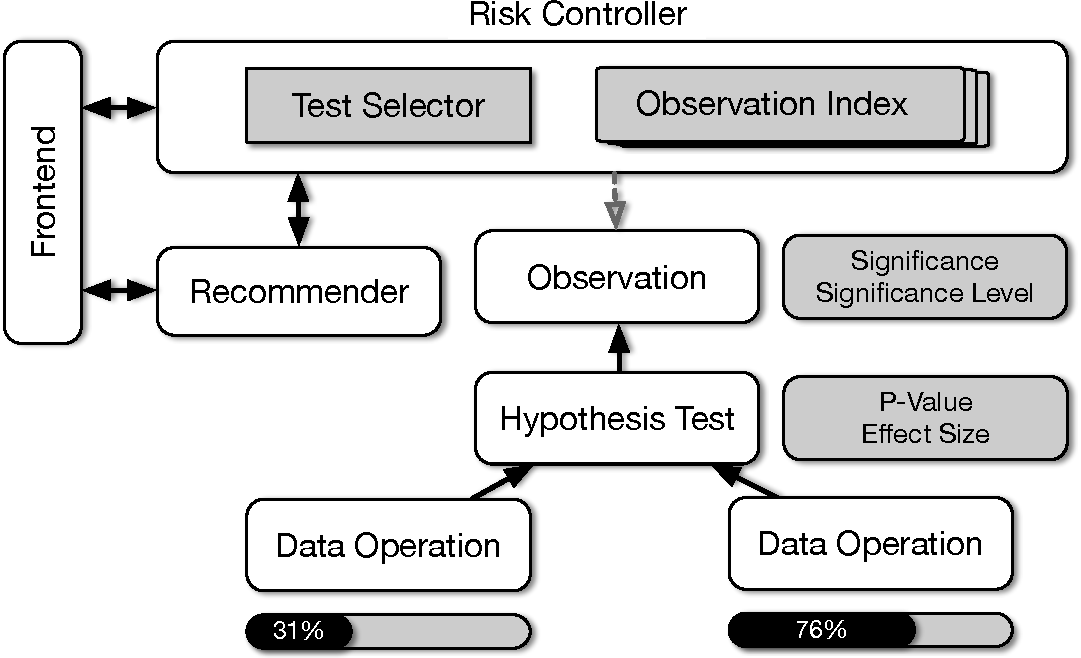
\includegraphics[scale=0.4]{figures/risk-controller.pdf}
\caption{Backend Risk Controller}
\label{fig:backend}	
\end{figure}

The highlight of the \system{} backend is the distributed and parallel computation of data-driven observations while preserving the linear ordering necessary for the false discovery procedures introduced in~\cite{zhao2016controlling}.  Our design combines functional reactive programming~\cite{wan2000functional} and progressive approximation paradigm~\cite{onlineagg,zgraggen2016progressive,vizdom} to dataflow processing to achieve practical interactivity and scalability.

The central piece of the \system{} backend is the \textit{risk controller} that implements the false discovery control procedures as introduced in~\cite{zhao2016controlling}.  Figure~\ref{fig:backend} highlights the design.  A risk controller bootstraps with a predefined exploration budget on a new dataset and invests a fraction on each observation, as described in Section~\ref{sec:theory}.  Observations are created by either the frontend user manually or the backend recommender.  Observations are tracked and indexed by the risk controller to make global decisions on each observation's appropriate significance level and its significance. A loose analogy of the observation index is perhaps a version control system, such as Git~\cite{torvalds2010git}, but in this case for data-driven observations. Such design allows distributed and parallel computation of observations for better performance, yet meanwhile enforces a linear ordering for the false discovery control procedures in~\cite{zhao2016controlling}. The observation index can also be used to look up the same observations for different frontend users or the backend recommender. 

An observation is a comparison of two distributions based on different conditions.  A comparison, for example, can be of the means, variances, correlations or histogram frequencies. Each observation is formulated as a null and an alternative hypothesis.  The risk controller is responsible of choosing the appropriate hypothesis test based on a given observation.  For example, to compare two means being different, a two-sided $t$-test is chosen; $\chi^2$-test is used to compare two histograms, but only when the frequencies are large enough; whereas for small frequencies, a permutation test is used. 

An data operation, on the other hand, extracts information from the underlying data source.  For example, an ``EmpiricalDistOperation'' calculates the mean and variance on the given attribute; whereas a ``HistogramOperation'' constructs bins and frequencies from some attribute.  Filters are pushed down to data operations.

\system{} implements the reactive programming~\cite{wan2000functional} and progressive approximation paradigm~\cite{vizdom, zgraggen2016progressive}. \system{} composes operations into dataflow that is reactive, where approximate updates are pushed as a stream from observed to observer operations. For example, an observation depends on its underlying hypothesis test, which then depends on the data operations. Data operations computes approximate information about the data source based on sampling, which eventually converges to the exact information as it completes the pass on the data source. The approximate information then forms an update stream that is pushed to any relevant hypothesis tests. A hypothesis test observes the approximate updates to calculate the effect sizes and \pvals, which in turn serve as the input to the risk controller to determine the significance of the observation progressively. 

Data updates can not be treated simply as re-evaluation of the observations, because this would reintroduce the multiple comparison problem.  To safely handle data updates, \system{} continues with its current exploration budget, if any, and for those observations whose underlying data operations overlap with the updated data, add them to the risk controller as if they were new observations.  Otherwise, if the exploration budget is already zero, the user and the recommender can reduce the per-observation investment for all the past observations, as stated in Section~\ref{sec:theory}.

\section{Scenarios}
\label{sec:scenarios}



\section{Conclusion}
\label{sec:conclusion}
Visual data exploration and recommendation examines large number of observations, and if not correctly controlled, would mistake visually significant results as statistically significant.  Recent theoretical advance in multiple comparison problem and control procedures adds the desirable property of interactivity to data exploration~\cite{zhao2016controlling}.  \system{} implements these interactive procedures. The pen-and-touch userface interface provides a smooth user experience.  The \system{} backend combines functional reactive programming and progressive approximation to achieve practical interactivity and scalability.

%\section{Acknowledgments}
%This research is funded in part by the Intel Science and Technology Center for Big Data, the NSF CAREER Award IIS-1453171, the Air Force YIP AWARD FA9550-15-1-0144, NSF IIS-1514491, and gifts from SAP, Oracle, Google, Mellanox, and Amazon.

%\clearpage
\balance
\begin{scriptsize}
\bibliographystyle{abbrv}
\bibliography{bib}
\end{scriptsize}

\end{document}